\documentclass{standalone}
\usepackage{tikz}
\usetikzlibrary{calc,arrows}
\usepackage{verbatim}
\usepackage{pgfplots}
\usepackage{gensymb}
\usetikzlibrary{positioning}

% argument #1: any options
\newenvironment{customlegend}[1][]{%
    \begingroup
    % inits/clears the lists (which might be populated from previous
    % axes):
    \csname pgfplots@init@cleared@structures\endcsname
    \pgfplotsset{#1}%
}{%
    % draws the legend:
    \csname pgfplots@createlegend\endcsname
    \endgroup
}%
% makes \addlegendimage available (typically only available within an
% axis environment):
\def\addlegendimage{\csname pgfplots@addlegendimage\endcsname}

\pgfplotsset{compat=1.15}
\begin{document}

\tikzset{font={\fontsize{15pt}{15}\selectfont}}
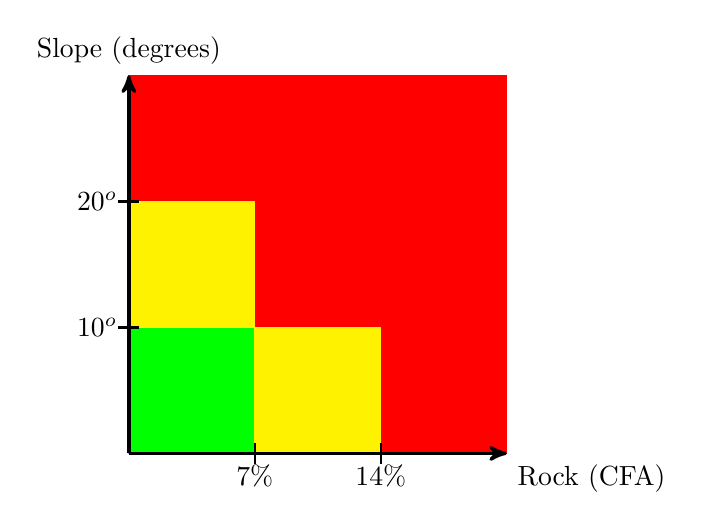
\begin{tikzpicture}[
        %We set the scale and define some styles
        scale=1.5,
        axis/.style={very thick, ->, >=stealth'},
        important line/.style={thick},
        dashed line/.style={dashed, thick},
        every node/.style={color=black}
    ]
    % Important coordinates are defined
    \newcommand\x{3.2}

    %We make some nice shading to annotate different parts of the curve
    %  Stop
    \draw [fill=red,red] (0,0) rectangle (\x,\x);
    
    % High Speed
    \begin{scope}
    \draw [fill=green,green] (0,0) rectangle (\x/3,\x/3);
    \end{scope}
    % Low Speed
    \begin{scope}
    \draw [fill=yellow,yellow] (0,\x/3) rectangle (\x/3,2*\x/3);
    \draw [fill=yellow,yellow] (\x/3,0) rectangle (2*\x/3,\x/3);
    \end{scope}
    % Axis
    \begin{scope}
    \draw[axis] (0,0)  -- (\x,0) node(xline)[below right]{Rock (CFA)};
    \draw[axis] (0,0) -- (0,\x) node(yline)[above]{Slope (degrees)};
    \end{scope}
    % Cordinates
    \draw[thick] (\x/3,-2.5pt) -- (\x/3,2.5pt) node[below=0.15] {7\%};
    \draw[thick] (2*\x/3,-2.5pt) -- (2*\x/3,2.5pt) node[below=0.15] {14\%};
    \draw[thick] (-2.5pt,\x/3) -- (2.5pt,\x/3) node[left=0.15] {10$^{o}$};
    \draw[thick] (-2.5pt,2*\x/3) -- (2.5pt,2*\x/3) node[left=0.15] {20$^{o}$};
    
    % \begin{customlegend}[
    % legend entries={High Speed, Low Speed, Stop},
    % legend style={at={(\x,\x)}, font={\fontsize{7pt}{7}\selectfont}}]
    % % the following are the "images" and numbers in the legend
    % \addlegendimage{area legend,green,fill=green}
    % \addlegendimage{area legend,yellow,fill=yellow}
    % \addlegendimage{area legend,red,fill=red}
    % \end{customlegend}
\end{tikzpicture}
\end{document}